% Nallino, Part I p. 254, the figure on the left: Schiaparelli's construction of formula (alpha), redrawn
% from the print: the epicycle about A, the line from its top H through M and A to F and the Earth E, the line
% from G to E, the radius AG and the perpendicular MG, and the bold italic letters. Measured on the scan
% (_intake/latin/tools/fig254).
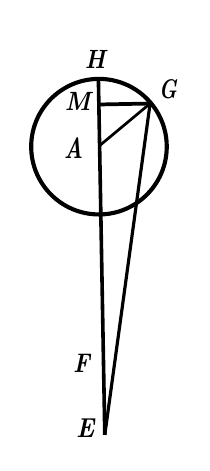
\begin{tikzpicture}[x=0.9928pt,y=-0.9928pt,line cap=butt,every node/.style={font=\fontsize{11}{11}\bfseries\itshape\selectfont,inner sep=0pt}]
\useasboundingbox (0,0) rectangle (56.00,151.00);
\draw[line width=1.49pt] (25.95,43.31) circle[radius=24.67];  % the epicycle about A
\draw[line width=1.30pt] (25.74,18.63) -- (28.07,148.23);  % the line from H through M, A and F to the Earth E
\draw[line width=1.15pt] (44.56,27.61) -- (28.07,148.23);  % the line from G to E
\draw[line width=0.99pt] (26.18,42.93) -- (44.56,27.61);  % the radius AG
\draw[line width=1.35pt] (25.91,27.96) -- (44.56,27.61);  % the perpendicular MG
\node at (24.51,11.42) {\normalfont\fontsize{11}{11}\bfseries\itshape\selectfont \resizebox{7.40pt}{6.54pt}{H}};
\node at (18.22,26.98) {\normalfont\fontsize{11}{11}\bfseries\itshape\selectfont \resizebox{9.29pt}{6.55pt}{M}};
\node at (51.05,22.58) {\normalfont\fontsize{11}{11}\bfseries\itshape\selectfont \resizebox{6.57pt}{6.69pt}{G}};
\node at (16.68,44.08) {\normalfont\fontsize{11}{11}\bfseries\itshape\selectfont \resizebox{6.95pt}{7.25pt}{A}};
\node at (19.59,122.02) {\normalfont\fontsize{11}{11}\bfseries\itshape\selectfont \resizebox{6.04pt}{6.66pt}{F}};
\node at (20.91,145.68) {\normalfont\fontsize{11}{11}\bfseries\itshape\selectfont \resizebox{6.59pt}{6.79pt}{E}};
\end{tikzpicture}
